%
% Main document
% ===========================================================================
% This is part of the document "Project documentation template".
% Authors: brd3, kaa1
%

%---------------------------------------------------------------------------
\documentclass{bfh_template}
\usepackage{tikz}
\usetikzlibrary{arrows,shadows}
\usepackage{pgf-umlsd}

%---------------------------------------------------------------------------
%  Read title, version number and date of the paper from the file:
%  title_version_def.tex
\providecommand{\titel}{Metropolitan-Sensor/Aktor-Netze unter Einsatz von LoRa und anderen Techniken}					%  Hier den Titel des Berichts/Thesis eingeben
\providecommand{\versionnumber}{1.0}			%  Hier die aktuelle Versionsnummer eingeben
\providecommand{\versiondate}{25.06.2016}		%  Hier das Datum der aktuellen Version eingeben


%---------------------------------------------------------------------------
\begin{document}                        % Start Document


%---------------------------------------------------------------------------
% Title Page and Abstract
%---------------------------------------------------------------------------
%\include{lead/titelseite_ohne_bild}	% activate for Titelseite ohne Bild
%
% Project documentation template
% ===========================================================================
% This is part of the document "Project documentation template".
% Authors: brd3, kaa1
%

\begin{titlepage}


% BFH-Logo absolute placed at (28,12) on A4 and picture (16:9 or 15cm x 8.5cm)
% Actually not a realy satisfactory solution but working.
%---------------------------------------------------------------------------
\setlength{\unitlength}{1mm}
\begin{textblock}{20}[0,0](28,12)
	
\includegraphics[scale=1.0]{pictures/BFH_Logo_B.png}
\end{textblock}

\begin{textblock}{154}(28,48)
	\begin{picture}(150,2)
		\put(0,0){\color{bfhgrey}\rule{150mm}{2mm}}
	\end{picture}
\end{textblock}

\begin{textblock}{154}[0,0](28,50)
	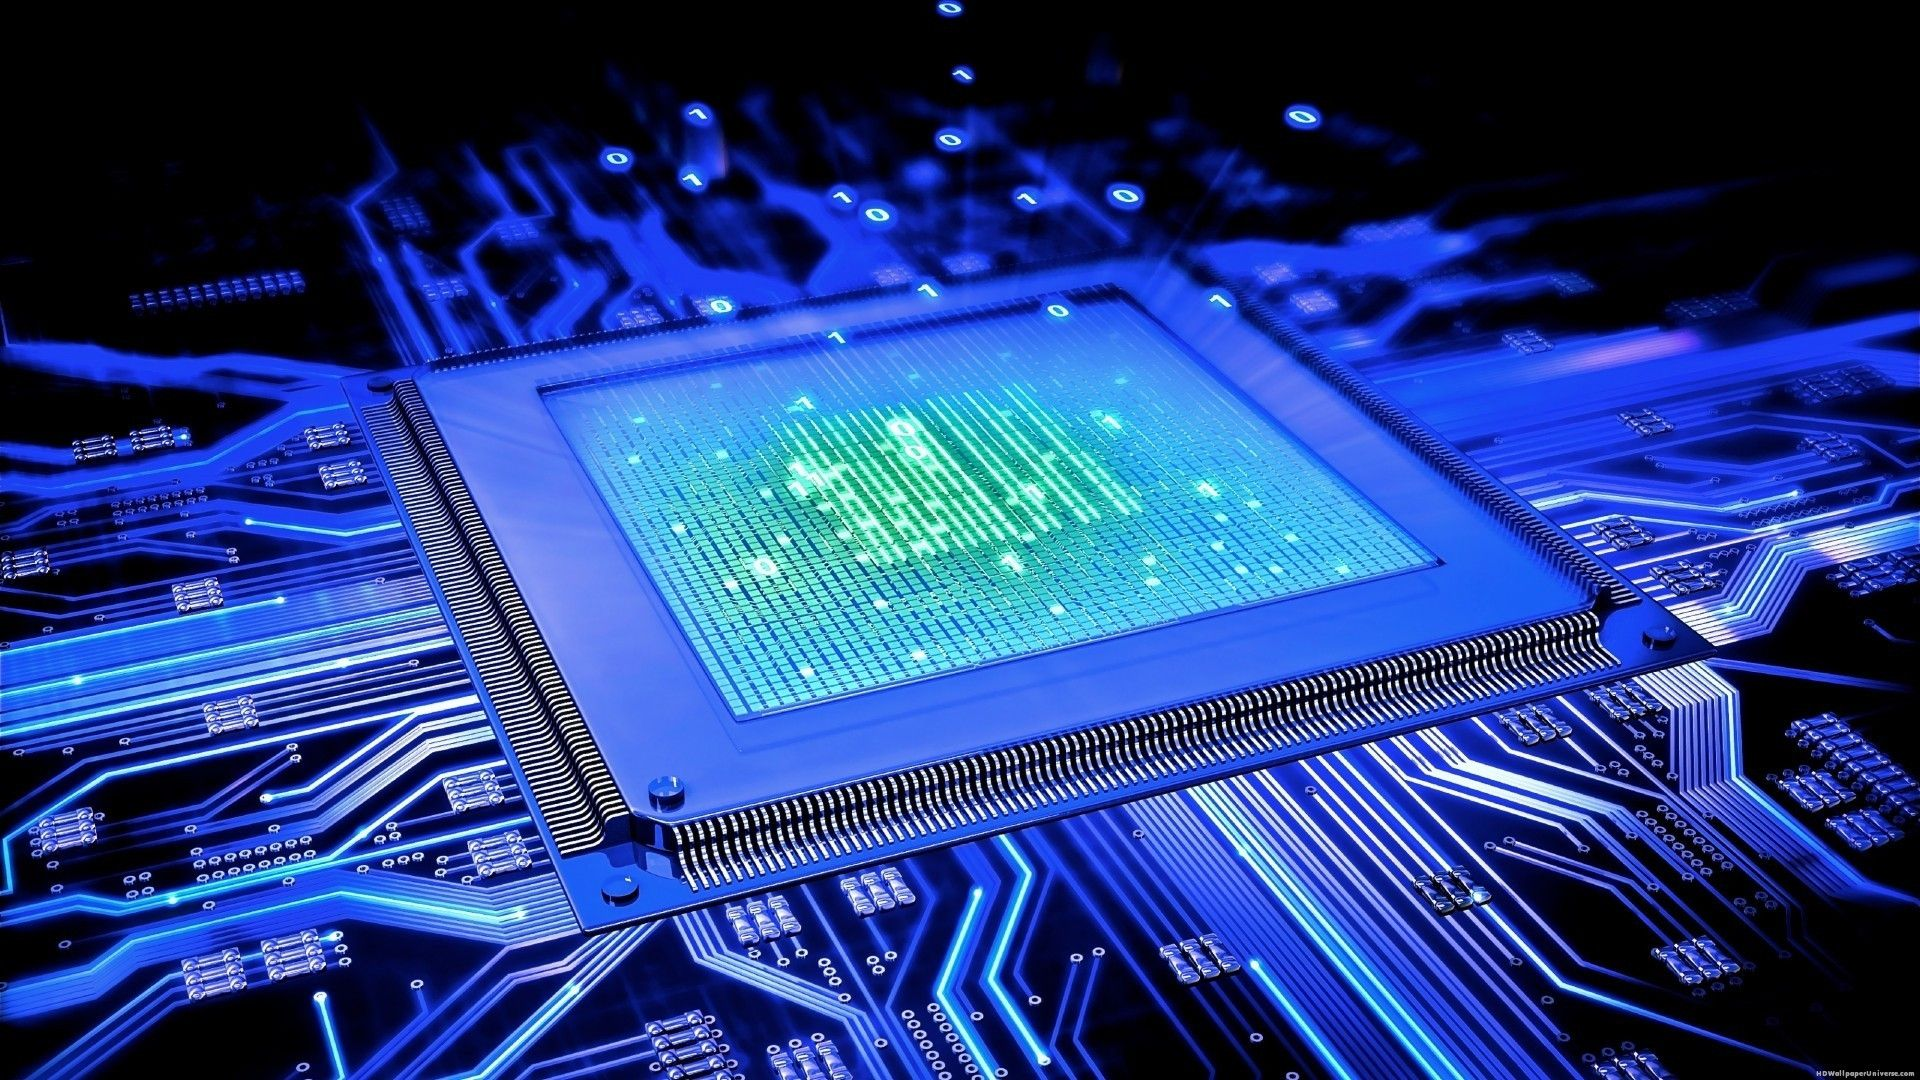
\includegraphics[height=85mm,width=150mm]{pictures/cs.jpg}
%\includegraphics[width=150mm]{pictures/network-782707_1280.png}			% Titelbild definieren
%1.764705882
\end{textblock}

\begin{textblock}{154}(28,135)
	\begin{picture}(150,2)
		\put(0,0){\color{bfhgrey}\rule{150mm}{2mm}}
	\end{picture}
\end{textblock}
\color{black}

% Institution / Titel / Untertitel / Autoren / Experten:
%---------------------------------------------------------------------------
\begin{flushleft}

\vspace*{115mm}

\fontsize{26pt}{28pt}\selectfont
\titel 								\\ % Titel aus der Datei lead/titel.tex lesen
\vspace{2mm}

% \fontsize{16pt}{20pt}\selectfont\vspace{0.3em}
% Subtitle 	\\ % Untertitel eingeben
% \vspace{5mm}

\fontsize{10pt}{12pt}\selectfont
\textbf{Projekt 2} \\ % eingeben
\vspace{3mm}

% Abstract (eingeben):
%---------------------------------------------------------------------------
%\begin{textblock}{150}(28,190)
%\fontsize{10pt}{12pt}\selectfont
%[Kurztext (Abstract) einfügen, falls gewünscht] \\
%Dieses Dokument dient als Vorlage für die Erstellung von Berichten nach den Richtlinien der BFH. Die Vorlage ist %in \LaTeX{} erstellt und unterstützt das automatische Erstellen von diversen Verzeichnissen, Literaturangaben, %Indexierung und Glossaren. Dieser kleine Text ist eine Zusammenfassung über das vorliegenden Dokument mit einer %Länge von 4 bis max. 8 Zeilen. \\
%Das Titelbild kann in den Zeilen 157/158 der Datei template.tex ein- oder ausgeschaltet werden.
%\end{textblock}

\begin{textblock}{150}(28,225)
\fontsize{10pt}{17pt}\selectfont
\begin{tabbing}
xxxxxxxxxxxxxxx\=xxxxxxxxxxxxxxxxxxxxxxxxxxxxxxxxxxxxxxxxxxxxxxx \kill
\\
\\
Studiengang:	\> Bachelor of Science Informatik	\\	% Namen eingeben
Autor:			\> Simon Wittwer, Marc Zimmermann	\\	% Namen eingeben
Betreuer:		\> Dr.~Andreas Danuser				\\	% Namen eingeben
% Experte:		\> Don Mutex						\\	% Namen eingeben
Datum:			\> \versiondate						\\	% aus Datei lead/versions.tex lesen
\end{tabbing}

\end{textblock}
\end{flushleft}

\begin{textblock}{150}(28,280)
\noindent
\color{bfhgrey}\fontsize{9pt}{10pt}\selectfont
Berner Fachhochschule | Haute école spécialisée bernoise | Bern University of Applied Sciences
\color{black}\selectfont
\end{textblock}


\end{titlepage}

%
% ===========================================================================
% EOF
%
				% activate for Titelseite mit Bild
% Versionenkontrolle :
% -----------------------------------------------

\null
\vfill

\begin{Large}
Versionen
\end{Large}

\fontsize{10pt}{18pt}\selectfont
\begin{tabbing}
xxxxxxxxxxx\=xxxxxxxxxxxxxxx\=xxxxxxxxxxxxxx\=xxxxxxxxxxxxxxxxxxxxxxxxxxxxxxxxxxxxxxxxxxxxxxx \kill
Version	\> Datum	\> Status		\> Bemerkungen		\\
0.1	\> 22.04.2016	\> Entwurf		\> Latex-Dokument eingerichtet	\\
0.1.1\> 23.04.2016	\> Entwurf		\> Kapitelstruktur erstellt \\
0.2	\> 12.06.2016	\> Entwurf		\> Anforderungen \\
0.3	\> 11.06.2016	\> Entwurf		\> Kapitel Einleitung \\
0.4	\> 18.06.2016	\> Entwurf		\> Kapitel Anwendungsfälle und Anforderungen \\
0.5	\> 20.06.2016	\> Entwurf		\> Kapitel Rahmenbedingungen \\
0.6	\> 20.06.2016	\> Entwurf		\> Kapitel Use Case Tresh \\
0.7	\> 23.06.2016	\> Entwurf		\> Kapitel Drahtlose Datenübertragung \\
0.8	\> 24.06.2016	\> Entwurf		\> Kapitel Prototyp, Resultate, Anhang \\
0.9	\> 25.06.2016	\> Entwurf		\> Management Summary, Fazit und Korrektur lesen \\
1.0	\> 25.06.2016	\> Final		\> Finale Version \\
\end{tabbing}


\cleardoubleemptypage
%\setcounter{page}{1}

\cleardoublepage
\phantomsection
% % \chapter*{Summary}\label{summary}
% \addcontentsline{toc}{chapter}{Summary}

\begin{abstract}
{\huge Management Summary\par} % parens are here to define the scope of \huge and \par
% \lipsum[1]
Diese Arbeit befasst sich im Rahmen des Projekt 2 mit verschiedenen Aspekten von \gls{iot}. Einerseits wird versucht mit der Auseinandersetzung von möglichen Use-Cases über verschiedene Branchen hinweg, ein Gefühl für das Marktpotential und die Herausforderungen von \gls{iot} zu entwickeln und daraus gleichzeitig wichtige Anforderungen an \gls{iotk} abzuleiten. Andererseits wird mit der Gegebüberstellung der wichtigsten Funktechnologien und deren Vor- und Nachteilen eine Übersicht verschafft und die auf Spreizbandmodulation basierende Technologie \gls{lora} vertieft betrachtet.\\
Um die verschiedenen Aspekte schliesslich zu kombinieren, wird der konkrete Use-Case \glqq{}Tresh\grqq{} vorgestellt und dessen Implementation und die gewonnenen Erfahrungen anhand eines Prototypen aufgezeigt.
\end{abstract}

% \chapter*{Summary}\label{summary}
% \addcontentsline{toc}{chapter}{Summary}

\begin{abstract}
{\huge Management Summary\par} % parens are here to define the scope of \huge and \par
% \lipsum[1]
Diese Arbeit befasst sich im Rahmen des Projekt 2 mit verschiedenen Aspekten von \gls{iot}. Einerseits wird versucht mit der Auseinandersetzung von möglichen Use-Cases über verschiedene Branchen hinweg, ein Gefühl für das Marktpotential und die Herausforderungen von \gls{iot} zu entwickeln und daraus gleichzeitig wichtige Anforderungen an \gls{iotk} abzuleiten. Andererseits wird mit der Gegebüberstellung der wichtigsten Funktechnologien und deren Vor- und Nachteilen eine Übersicht verschafft und die auf Spreizbandmodulation basierende Technologie \gls{lora} vertieft betrachtet.\\
Um die verschiedenen Aspekte schliesslich zu kombinieren, wird der konkrete Use-Case \glqq{}Tresh\grqq{} vorgestellt und dessen Implementation und die gewonnenen Erfahrungen anhand eines Prototypen aufgezeigt.
\end{abstract}

\cleardoubleemptypage

%---------------------------------------------------------------------------
% Table of contents
%---------------------------------------------------------------------------
\tableofcontents

%---------------------------------------------------------------------------
% Main part
%---------------------------------------------------------------------------
\cleardoublepage
\pagenumbering{arabic}
\chapter{Einleitung}

\acrfull{iot} hat laut Gartner gerade den Höhepunkt des Hypes erreicht. Der Begriff ist in aller Munde und jeder kennt es. Doch wo sind solche "Things" tatsächlich bereits anzutreffen? Diese Arbeit behandelt das Thema "Metropolitan-Sensor/Aktor-Netze unter Einsatz von LoRa und anderen Techniken". Sie sucht nach Anwendungsfällen wo solche Things, auch \gls{iotk} genannt, im urbanen Umfeld sinnvoll eingesetzt werden können.\\
Ein \gls{iotk} ist ein Mikrocontroller, welcher Sensoren und Aktoren verwaltet. Die Sensordaten sendet er über eine Verbindung zu einem Gateway, welches die Daten wiederum an einen Server oder in die Cloud leitet. Umgekehrt können vom Server oder von der Cloud Befehle über das Gateway an den Controller geschickt werden. Der Controller steuert damit die Aktoren. Aus solchen \gls{iotk} und  Gateways entsteht schliesslich ein Sensor-Aktor-Netz. Für dieses Netz spielt die Verbindung zwischen den IoT-Knoten und den Gateways eine sehr wichtige Rolle. Sie definiert Faktoren wie Distanz, Bandbreite und Energieverbrauch. Diese Faktoren sind für einen \gls{iotk} von entscheidender Bedeutung da sie direkten Einfluss auf dessen Lebensdauer und seine Kosten haben. Ebenso beschränkt es die Grösse des Netzes, je nachdem welche Reichweite mit der Verbindung möglich ist. Da die \gls{iotk} oft an Orten eingerichtet werden wo weder eine Netzwerk-Anbindung noch Energieversorgung verfügbar ist, muss der Sensor möglichst autark sein. Das bedingt eine drahtlose Verbindung zwischen der Knoten und der Gateways. Aus diesem Grund behandelt die Arbeit unter anderem verschiedene Funk-Standards, welche zurzeit existieren und in den Frequenzen eines \gls{ism}es sind, damit keine Lizenzen die Kosten der \gls{iotk} in die Höhe treiben. LoRa, eine Funkmodulationstechnik hat seine Stärken genau in den Faktoren Distanz und Energieverbrauch, weshalb sie ideal für solche Verbindungen geeignet scheint. Aus diesem Grund implementiert diese Arbeit ein Proof-of-concept mit diesem Standard. 
\chapter{Anwendungsfälle für IoT}

\chapter{Rahmenbedingungen für \gls{iot}} \label{Rahmenbedingungen für iot}
Die Use Cases aus den verschiedensten Branchen zeigen: in praktisch jeder Lebenssituation können Dinge automatisiert oder verbessert werden. So manchen Prozess, welchen wir heutzutage regelmässig wiederholen, kann automatisiert oder zumindest zeitlich optimiert werden, so dass er nur ausgeführt wird, wenn er wirklich nötig ist. Viele der beschriebenen Use Cases sind von mehreren Faktoren Abhängig. Der in Smart Home beschriebene Wecker benötigt beispielsweise folgende Sensoren und Aktoren:
\begin{itemize}  
  \item Zeit-Sensor (Real-Time Clock)
  \item Wetter-Sensor (Licht-Sensor vor dem Fenster)
  \item Schlafphasen-Sensor (Smartwatch)
  \item Aufsteh-Sensor (Bodenplatten-Sensoren oder Smartwatch)
  \item Storen-Aktor (Elektrisch gesteuerte Storen)
  \item Licht-Aktor (Smarte LEDs)
  \item Musik-Aktor (Smarte Stereoanlage)
\end{itemize}
Dieser Wecker funktioniert erst, wenn der Wecker alle diese Sensoren auslesen kann und die Aktoren steuern kann. Natürlich könnte ein Wecker konstruiert werden, welcher all diese Informationen für sich erfasst und so autonom funktioniert. Es existieren mittlerweile auch bereits alle Sensoren und Aktoren für sich. Allerdings wäre ein solch intelligenter Wecker als Komplettprodukt viel zu teuer und nicht erweiterbar. Deshalb ist es viel sinnvoller, wenn Sensoren ihre Daten an eine \gls{iotp} senden, welche die Sensordaten über standardisierte Schnittstellen empfängt und danach für Aktoren wieder über Schnittstellen bereitstellt. Erst mit einer solchen Plattform kann \gls{iot} sein Potential ausschöpfen. Durch das Teilen von Informationen können Sensoren und Aktoren voneinander profitieren.
Somit muss nicht jedes System seine eigenen Sensoren und Aktoren zur Verfügung stellen. Redundanzen können verhindert werden. Dies ermöglicht, dass komplexe Systeme rasch und effizient entstehen können.  

\section{\gls{iotk}}
Heutzutage existieren bereits viele Sensoren und Aktoren. Beispielsweise haben die meisten aktuellen Smartphones Sensoren für Helligkeit, Temperatur, Beschleunigung Neigung, Position, Feuchtigkeit und Näherung. Leider befinden sich Smartphones einem grossen Teil der Zeit in Hand- oder Hosentaschen, weshalb die Sensoren für die meisten Anwedungsfälle keine sinnvollen Daten messen. Weiter verwenden  Smartphones die Kostenpflichtigen 2/3/4G-Netzwerke. Dies ist finanziell nicht interessant und energetisch nicht sinnvoll, da diese Netzwerke nicht für Niedrigst-Energie-Geräte entwickelt wurden. Aus diesen Gründen eignen sich Smartphones eher schlecht als \gls{iotk}. Damit ein \gls{iotk} sinnvoll eingesetzt werden kann, sollte er nur die nötigsten Sensoren haben und diese müssen sinnvoll positioniert sein, damit sie die Daten für den Use Case optimal ermitteln können. Statt also auf ein mit Sensoren vollgepacktes Gerät, wie ein Smartphone, aufzusetzen, macht es mehr Sinn neue Sensor-Knoten zu bauen, welche speziell auf einen Use Case abgestimmt sind.

\section{\gls{iotp}}
Wie bereits erwähnt brauchen die \gls{iotk} eine zentrale Stelle, welche die Sensordaten entgegennimmt und bei bedarf speichern, aggregieren oder manipulieren kann. Das Unterenehmen Appmodule entwickelt unter der Leitung von Andreas Danuser eine solche Plattform. 
\subsection{SIOT.net}
SIOT.net bietet Schnittstellen via MQTT, WebSocket sowie REST um Sensor-Daten entgegenzunehmen. Zugleich bietet Sie die Möglichkeit mit Node-Red, die Daten zu aggregieren und Events auszulösen oder Aktoren zu steuern. Weiter bietet sie eine Art Dashboard in welcher die Sensorwerte präsentiert werden können.

\section{\gls{iotg}}
Zur Verbindung der \gls{iotk} und der \gls{iotp} wird schliesslich ein Gateway benötigt. Dieses empfängt die Funkdaten verschiedener Knoten und sendet sie an die Plattform mit zusätzlichen Informationen wie Beispielsweise der Sensor-ID oder der Empfangsqualität des Empfangenen Pakets. Das Gateway ist somit einerseits ein Übersetzer von \gls{iot}-Kommunikation zu klassischer Netzwerk-Kommunikation, andererseits hat es auch noch eine Sensor-Funktion, da es den Zustand der Kommunikation und des \gls{iot}-Netzes an die Plattform meldet. 

\begin{figure}[H]
    \centering
        \includegraphics[width=1.0\textwidth]{pictures/IoT_Conditions.png}
    \caption{IoT Module}
    \label{fig:IoT Module}
\end{figure}


\chapter{Anforderungen an \gls{iotk}}

Durch das Analysieren von Anwendungsfällen im vorherigen Kapitel, haben sich wichtige Anforderungen an \gls{iotk} herauskristallisiert. Nachfolgend werden diese genauer beschrieben.

\section{Reichweite}

Je nach Anwendungsfall gibt es unterschiedliche Anforderungen an die Reichweite eines \gls{iotk}. Die flexibelste Art Daten zu Senden und Empfangen ist über eine drahtlose Funkverbindung. Bei kurzen Distanzen und vorhandener Energieversorgung genügen oft konventionelle Technologien wie \gls{wifi} oder \gls{bluetooth}. Sobald aber die Distanzen zwischen den \gls{iotk} grösser werden und zusätzlich noch Hindernisse wie Gebäude oder Hügel überwunden werden müssen, werden andere Technologien benötigt. Die Funkmodulationstechnik \gls{lora} erlaubt das Übertragen von Daten über mehrere Kilometer, doch nicht ohne dabei einen Kompromiss einzugehen. Grundsätzlich gilt: Je tiefer die Übertragungsfrequenz desto grösser ist die Reichweite und umso kleiner ist der Datendurchsatz. Das heisst bei \gls{lora} kann eine Vergrösserung der Reichweite auf Kosten des Datendurchsatzes erreicht werden. Die physikalischen Gesetze zwingen zu einem Abwägen zwischen Reichweite und Datendurchsatz bei der Wahl der geeigneten Funk-Technologie für ein Sensor/Aktor Netzwerk. Diese Tatsache hat noch weitere Implikationen auf andere Anforderungen wie Verwaltbarkeit und Datendurchsatz.

\section{Datendurchsatz}

Je nach dem wie viele Daten in einem Sensor/Aktor Netzwerk anfallen, wird ein unterschiedlicher Datendurchsatz benötigt. Wie im oberen Abschnitt beschrieben beeinflusst der Datendurchsatz die mögliche Reichweite und somit die Wahl der geeigneten Technologien. Über eine \gls{wifi} 802.11n Verbindung können bis zu 300Mbs übertragen werden, d.h. Bild- , Audio- und Videodaten können ohne Probleme in kurzer Zeit übertragen werden. Sogar das Streaming von hochauflösenden Videodaten ist möglich. Im Gegensatz dazu ist es in einem \gls{lora}-Netzwerk äusserst ineffizient Bilddaten zu übertragen und undenkbar Videostreaming zu betreiben, denn die maximale Datenrate von \gls{lora} (Mode 10) beträgt 38.4kbps \autocite[2]{lora:FAQ}.\\
Ein weiterer Faktor der den Datendurchsatz beeinflusst ist die Anzahl Teilnehmer in einem Netz die gleichzeitig Daten versenden. Wenn nur ein einzelner Knoten Daten versendet, kann er die volle Datenrate ausnutzen. Mit jedem weiteren Teilnehmer der dazu kommt, muss die Datenrate geteilt werden.\\
Bei der Wahl eines \gls{iotk} ist der Datendurchsatz also ein wichtiges Entscheidungskriterium. Je nach Anwendungsfall muss zischen Datendurchsatz, Reichweite und Anzahl Teilnehmer im Netzwerk abgewogen werden.

\section{Zuverlässigkeit}

Eine weitere wichtige Anforderung an einen \gls{iotk} ist seine Zuverlässigkeit. Grundsätzlich ist hiermit der Determinismus des Systems gemeint, also dass sich das System immer gleich verhält und dieses Verhalten klar bestimmt ist. Konkret müssen folgende Kriterien eines \gls{iotk} Zuverlässig sein:
\begin{itemize}  
  \item Messresultate der Sensoren
  \item Funktion der Aktoren
  \item Übertragung der Daten
  \item Übertragungszeit im Netzwerk (Jitter)
  \item Entladekurve der Energiespeicher
\end{itemize}

Mit einer hohen Zuverlässigkeit kann ein System optimal operieren, insbesondere über einen längeren Zeitraum. Der Wartungsaufwand kann minimiert und genauer geplant werden. Da durch den deterministischen Charakter einige Parameter des Systems berechenbar werden, lassen sich daraus leicht einige Annahmen ableiten.

\section{Sicherheit}

Die Frage nach der Sicherheit eines Systems ist ein Dauerbrenner in der Informationstechnologie. So auch im \acrshort{iot}-Sektor. Je nach dem wie sensibel die Daten sind, die mit einem \gls{iotk} gemessen und übertragen werden, müssen andere Sicherheitsmassnahmen getroffen werden. Die \gls{iotk} sollten eine eingebaute Hardwarebeschleunigung für kryptographische Operationen unterstützten, wie z.B. AES-Beschleunigung. Für hochsensible Daten ist die Möglichkeit der End-zu-End Verschlüsselung vom Sensor bis zum Endnutzer nötig, was die Komplexität des Systems massiv erhöhen kann. Auch hier muss anhand der Anforderungen der Anwendung zwischen mehr Sicherheit oder mehr Akkulaufzeit (da keine zusätzlichen Chips für die Hardwarebeschleunigung benötigt werden) und Flexibilität abgewogen werden.

\section{Topologie}

Je nach Anwendungsgebiet und verwendeter Technologie sind unterschiedliche Netzwerk Topologien sinvoll. Die einfachste Topologie ist eine Punkt-zu-Punkt Verbindung. Dabei sind genau zwei Knoten miteinander verbunden. Während diese Topologie sehr einfach ist, ist sie gleichzeitig sehr eingeschränkt, da nur zwei Teilnehmer miteinander kommunizieren können. In einem Mesh Netzwerk leiten die Endknoten Daten von anderen Knoten weiter, um die Reichweite und die Anzahl Teilnehmer der Netzwerk-Zelle zu erhöhen. Dafür erhöht sich aber auch die Komplexität und Netzwerkkapazität. In einem Stern Netzwerk sind mehrere Teilnehmer mit einem zentralen \gls{iotg} verbunden. Die Teilnehmer können über dieses \gls{iotg} mit den anderen Teilnehmern kommunizieren. So kann viel Logik von den Knoten weg in das \gls{iotg} verschoben werden, was im Falle der \glspl{iotk} ein einfacheres Design erlaubt. Da es mehr \gls{iotk} als \glspl{iotg} gibt, hat dies auch einen Kosten-Nutzen.

\section{Energieverbrauch}

Ein kritischer Faktor für jeden \gls{iotk} ist der Energieverbrauch. Dieser ist von verschiedenen Faktoren wie Standort, Art und Anzahl Sensoren und Aktoren, Messintervallen und Operationen, verwendeter Hardwarekomponenten und verfügbarem Platz abhänging.\\
Ein idealer Standort eines Knotens hätte eine bereits vorhandene, stetige Energiequelle. Doch dies ist in der Praxis selten der Fall, da die Knoten oft an Orten mit keiner oder nur begrenzter Energieversorgung eingesetzt werden. Daher wird Platz für einen Energiespeicher benötigt. Optimal ist es, am Standort Energie zu gewinnen, beispielsweise mit Solarzellen. Der Energiespeicher ist somit ein Puffer, da die Gewinnung nicht konstant ist. \gls{iotk} werden oft in bestehende Systeme integriert, weshalb die Platzverhältnisse stark begrenzt sind. Diese knappen Verhältnisse schränken die Grösse des Energiespeichers und auch die Möglichkeiten der Energiegewinnung ein. Damit wird jedes Miliampere zu einem kostbaren Gut und ein haushälterischer Umgang damit verlängert die Lebensdauer und vermindert Wartungseinsätze.\\
Ein effizientes Energiemanagement kann mit dem Einsatz von auf den Anwendungsfall reduzierter Hardware, die es erlaubt in einen Energiesparmodus zu wechseln und dafür optimierter Software sichergestellt werden.

\subsection{Intelligente Messungen}

Um die gewünschten Informationen für die Anwendung mithilfe eines \glspl{iotk} zu ermitteln, sind auf den Anwendungsfall zugeschnittene, intelligente Messungen sehr wertvoll. Zwar könnte man einen Sensor so oft wie möglich auslesen und alle diese Werte über das Netzwerk in die Cloud speichern. Doch meistens ist dies gar nicht notwendig. Es erhöht nur unnötig den Energieverbrauch und die Auslastung des Netzwerks.\\
Je nach Anwendungsfall sind unterschiedliche Messarten sinnvoll. Diese können grundsätzlich in zwei Klassen aufgeteilt werden: Messungen können entweder durch einen Trigger oder zu definierten Zeitpunkten ausgelöst werden. Das ereignisbasierte Auslösen durch einen Trigger ist zum Beispiel beim Herausfinden ob eine Tür offen oder geschlossen ist sinnvoll. Nur die Zustandsänderung ist von Interesse, nicht aber eine dauernde Überwachung. Bei einer Anwendung wo es nicht möglich ist einen zuverlässiges Ereignis zu triggern, muss mit zeitzyklischen Messungen gearbeitet werden. Dabei muss bei der Bestimmung der Messintervalle zwischen Genauigkeit und Energieverbrauch abgewogen werden. Zusätzlich können Knoten während Zeiten, wo keine Messungen benötigt werden in den Energiesparmodus wechseln oder ganz abgeschaltet werden. Ein Beispiel dafür sind Alarmanlagen, sie müssen nur aktiv sein wenn kein Personal anwesend ist.

\section{Verwaltbarkeit}

Wenn einmal ein Netz von \gls{iotk} aufgebaut ist, stellt sich schnell einmal die Frage wie Änderungen an alle Knoten propagiert werden können. Je nach Topologie, Datendurchsatz und Intelligenz der Knoten bieten sich unterschiedliche Möglichkeiten an. Diese lassen sich in folgende vier Stufen aufteilen:

\begin{enumerate}
  \item Nur lokaler Zugriff
  \item Remote Reset des \gls{iotk}
  \item Remote Konfiguration einzelner Parameter des \gls{iotk}
  \item Remote \acrfull{ota}-Update 
\end{enumerate}

\section{Benutzerfreundlichkeit}

Je nachdem von welcher Zielgruppe schlussendlich die \glspl{iotk} verwendet werden, verändern sich auch die Anforderungen an die Benutzerfreundlichkeit der Knoten. Angenommen ein Parkhaus hat alle Parkfelder komplett neu mit Parksensoren ausgestattet. Der Abwart des Parkhauses ist neu für die Wartung aller Parksensoren verantwortlich. Seine Hauptaufgabe ist eine regelmässige Funktionskontrolle der Sensoren. Das Softwareunternehmen, welches das \acrshort{iot}-System entwickelt und integriert hat, ist verpflichtet das System weiter zu verbessern und will daher möglichst viel Kontrolle über die \gls{iotk} haben. Darum will das Unternehmen die Software möglichst Remote verwalten und aktualisieren können.
Die im vorderen Abschnitt erwähnten vier Stufen könnten wie folgt aussehen:

\textbf{Funktionskontrolle der Sensoren}
\begin{enumerate}  
  \item Der Abwart muss bei jedem \gls{iotk} vorbeigehen und eine Funktionskontrolle durchführen.
  \item Der Abwart kann zumindest versuchen einen defekten \gls{iotk} zuerst über eine Smartphone App zurückzusetzen, bevor er vorbeigehen muss.
  \item Der Abwart kann defekte \gls{iotk} über die Smartphone App identifizieren und gezielt reparieren.
  \item Der Abwart kann ein Zeitfenster definieren in welchem die Sensoren oder eine Sensorgruppe aktualisiert werden darf.
\end{enumerate}

\textbf{Software aktualisieren}
\begin{enumerate}  
  \item Das Untenehmen muss einen Mitarbeiter vorbeischicken der bei jedem \gls{iotk} vorbeigeht und von Hand flasht oder den Abwart instruieren.
  \item Wie Stufe 1.
  \item Die Entwickler können grosse Teile der Funktionalität ändern, wenn sie möglichst viel Logik in die \glspl{iotg} verlagern und auf den \gls{iotk} viele flexible Parameter definieren.
  \item Die Entwickler können die gesamte Software Remote ändern.
\end{enumerate}

\section{Kosten}

Ein entscheidender Faktor sind schlussendlich auch die Kosten. Der erste wichtige Kostenfaktor sind die Anschaffungskosten. Je tiefer der Preis pro \gls{iotk}, desto günstiger wird das Gesamtsystem. Wenn die Hardwarekomponenten genau auf den jeweiligen Anwendungsfall reduziert werden, können die Produktionskosten minimiert werden, was sich auf die Anschaffungskosten auswirkt. Dies hat auch meist auch positive Auswirkungen auf die Energieeffizienz der \gls{iotk}.\\
Ein weiterer Kostenfaktor sind die Wartungskosten. Umso länger ein \gls{iotk} zuverlässig läuft, desto weniger Kosten für die Wartung fallen an. Das heisst es können Personalkosten gespart werden, da sich niemand um defekte Knoten kümmern oder Akkumulatoren austauschen muss. Je länger und zuverlässiger ein \gls{iotk} ununterbrochen seinen Dienst verrichtet, desto weniger Betriebskosten fallen an. Ein zusätzlicher Kostenfaktor für den Betrieb ist die Wahl des Frequenzbandes. Wird zum Beispiel \gls{lora} eingesetzt, fallen gar keine Kosten für die Nutzung des Frequenzbandes an, da \gls{lora} ein \gls{ism} nutzt. Wird ein kostenpflichtiges Frequenzband eingesetzt, kann dies einen signifikanten Anteil an den Betriebskosten ausmachen. Ein letzter wichtiger Kostenfaktor ist die Zuverlässigkeit eines \gls{iotk} und ein möglichst geringer Verschleiss.

\chapter{Drahtlose Datenübertragung}

Der Bedarf an drahtlosen Technologien im industriellen sowie im privaten Umfeld steigt immer mehr. Die Schlüsselfaktoren, die hinter den Anforderungen für drahtlose Technologien stehen, sind zum einen die Fernsteuerung, damit verbunden die Mobilität und Flexibilität, zum anderen die verschleissfreie Übertragung von Daten. Beispielsweise können drahtlose Sensoren und Aktoren, die auf beweglichen Teilen von Maschinen positioniert werden, von Vorteil für drahtlose Systeme sein. Jede Anwendung hat unterschiedliche Anforderungen. Es gibt kein einzelnes drahtloses System, das alle Anforderungen gleichzeitig erfüllen kann.\\
Im Rahmen dieser Arbeit wurden mehrere Funktechnologien die im \acrshort{iot}-Umfeld in Frage kommen angeschaut und deren Vor- und Nachteile aufgezeigt, die nachfolgend beschrieben werden.

\section{BLE}

\section{BLE}
\chapter{Protoyp}


\include{chapters/demo.md}

%---------------------------------------------------------------------------
% Statement
%---------------------------------------------------------------------------
\cleardoublepage
\phantomsection
\addcontentsline{toc}{chapter}{Selbständigkeitserklärung}
\chapter*{Selbstständigkeitserklärung}
\label{chap:selbstaendigkeitserklaerung}

\vspace*{10mm}
Wir bestätigen mit unseren Unterschriften, dass wir unsere vorliegende Bachelorthesis selbstständig durchgeführt haben. Alle Informationsquellen (Fachliteratur, Besprechungen mit Fachleuten, usw.) und anderen Hilfsmittel, die wesentlich zu unserer Arbeit beigetragen haben, sind in unserem Arbeitsbericht im
Anhang vollständig aufgeführt. Sämtliche Inhalte, die nicht von uns stammen, sind mit dem genauen Hinweis auf ihre Quelle gekennzeichnet.

\vspace{15mm}

\begin{tabbing}
xxxxxxxxxxxxxxxxxxxxxxxxx\=xxxxxxxxxxxxxxxxxxxxxxxxxxxxxx\=xxxxxxxxxxxxxxxxxxxxxxxxxxxxxx\kill
Ort, Datum:		\> Bern, \versiondate \\ \\
Namen:	\> Simon Wittwer 	\> Marc Zimmermann \\ \\ \\ \\
Unterschriften:	\> ......................................\> ...................................... \\
\end{tabbing}


%---------------------------------------------------------------------------
% Glossary
%---------------------------------------------------------------------------
\cleardoublepage
\phantomsection
% \addcontentsline{toc}{chapter}{Glossar}
% \renewcommand{\glossaryname}{Glossar}
% \printglossary
\printglossaries

%---------------------------------------------------------------------------
% Bibliography
%---------------------------------------------------------------------------
\cleardoublepage
\phantomsection
% \nocite{*}
\addcontentsline{toc}{chapter}{Literaturverzeichnis}
% \bibliographystyle{IEEEtranS}
% \bibliography{references/bibliography}{}
\printbibliography


%---------------------------------------------------------------------------
% Listings
%---------------------------------------------------------------------------
\cleardoublepage
\phantomsection
\addcontentsline{toc}{chapter}{Abbildungsverzeichnis}
\listoffigures

\cleardoublepage
\phantomsection
\addcontentsline{toc}{chapter}{Tabellenverzeichnis}
\listoftables

%---------------------------------------------------------------------------
% Index
%---------------------------------------------------------------------------
%\cleardoublepage
%\phantomsection
%\addcontentsline{toc}{chapter}{Stichwortverzeichnis}
%\renewcommand{\indexname}{Stichwortverzeichnis}
%\printindex

%---------------------------------------------------------------------------
% Appendix
%---------------------------------------------------------------------------
\appendix
\settocdepth{section}
\include{appendix/example.md}


 % \includepdf[pages={-}]{../raspi/smoje/doc/latex/refman.pdf}
 % \clearpage
 % \addcontentsline{toc}{chapter}{Doxygen Smoje Code}
 % \includepdf[pages={-}]{appendix/smojeCodedoc.pdf}

%---------------------------------------------------------------------------
\end{document}
